\section{System test}
After the assembling of the PCB and testing the components behave like the expectation, the complete system test is performed. For the tests the PV simulator \textit{E4360} from Keysight Technologies \cite{PV_simulator} is used to simulate the PV panel \textit{STP300S-24/Vd} from Suntech Power \cite{PV_panel}. At first the converter is subjected the open-loop test. The reason of this test is to compare the measured voltages and current ripples with the values from the ideal open-loop simulation in appendix \ref{app:OL_ripple}. The second test includes the thermal test. For this test the converter is performed for a longer time to identify which parts of the PCB will be overheated. The last test is about validating the P\&O algorithm, if it behaves like in the simulation from section \ref{MPPTSimulation}.

\subsection{Open-loop test}

The open-loop test is carried out to measure the ripples in the inductor current, the input voltage and the output voltage of the converter. The test conditions were explained in section \ref{sec:componentsizing} and the graphs showing the experimental results are shown in appendix \ref{app:OL_ripple}.

The measured current ripple in the inductor is calculated from figure \ref{Openlooptestinductor} and shown in equation \ref{eq:inductor_ripple}. The minimum current is $I_{min} = 2.7A$ and the maximum current is $I_{max} = 2.98A$. The mean value for the inductor current is $\widebar{I_L}= 2.84$. 

\begin{equation} \label{eq:inductor_rippleexpirment}
\Delta I_L = \frac{I_{max}-I_{min}}{\widebar{I_L}} \cdot 100 = \frac{2.98A-2.7A}{2.84A} \cdot 100 = 9.86\%
\end{equation}

The result obtained for the output voltage ripple is shown in figure \ref{Openlooptestoutputtcapacitor}. The ripple percentage is calculated in equation \ref{eq:output_voltage_rippleexperiment} using the values obtained from the graph. 

\begin{equation} \label{eq:output_voltage_rippleexperiment}
\Delta V_{out} = \frac{V_{out,max}-V_{out,min}}{\widebar{V_{out}}} \cdot 100 = \frac{23.9082V - 23.895V }{23.9V} \cdot 100 = 0.055\%
\end{equation}

Finally, the measured input voltage ripple is shown in figure \ref{Openlooptestinputcapacitor}. It is observed from the figure that the signal is too noisy and it is not possible to identify the real voltage ripple. This is because the input voltage ripple was defined to be lower than 0.1\% and, as the input capacitor has a high capacitance, the measured ripple is neglected. \todo{check this and if it's necessary explain it better. Stef}

\subsection{Thermal test}

For this test, the converter is supplied for 10 minutes (or 600 seconds) a constant input voltage 36.9 V and input current 7 A. Tthe converter is performing in buck mode with the fix duty cycles D1 = 0.8 and D2 = 0 in this test. The temperature of the components coil, heat sink and security diode are measured during the test because they are the critical components. Figure \ref{Testthermal} shows that the diode is produced the most amount of heat.\todo {thats not true. This is only a random sentence.}

\begin{figure}[H]
	\begin{center}
		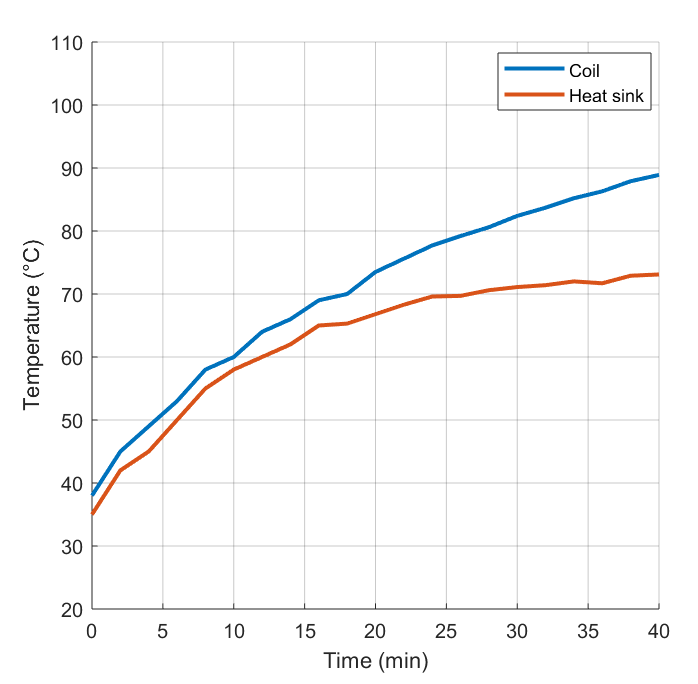
\includegraphics[width=0.65\textwidth]{../Pictures/P1/Test/Thermal_test_with_heat_sink}
		\caption{Thermal test.}
		\label{Testthermal}
	\end{center}	
\end{figure}

\subsection{MPPT test}
The MPPT test is divided in two parts as it was done for obtaining the simulation results. The test will be implemented for both modes of operation of the converter. For obtaining the results in buck mode a resistive load of 3$\Omega$ is used and, for boost mode, 27 $\Omega$.

 \subsubsection*{Standard Test Conditions (STC)}
For the first test, in both modes, the ambient condition is for irradiance 1000 $W /m^2$ and for temperature 25 $\decC$ (as STC). Figure \ref{MPPTtestbuckmode1} shows how the converter is tracking the MPP in buck mode. The left graph represents the input voltage and current of the converter. At first the input voltage reached the open circuit voltage as in the simulation.  After 10 seconds the P\&O algorithm reaches the MPP. The maximum average power obtained in the lab from the PV panel is 293.56 W. This can be seen in the right graph in figure \ref{MPPTtestbuckmode1}. By comparing the measured value of power with the maximum power that the PV panel can generate under these conditions, the performance of the MPPT can be quantified as shown in equation \ref{eq:effMPPTbuck}.

\begin{equation} \label{eq:effMPPTbuck}
\eta_{MPPT}= \dfrac{P_{pv}}{P_{mpp}} \cdot 100 = \dfrac{293.56W}{300.4W} \cdot 100 = 97.72\%  
\end{equation}


\begin{figure}[H]
	\begin{center}
		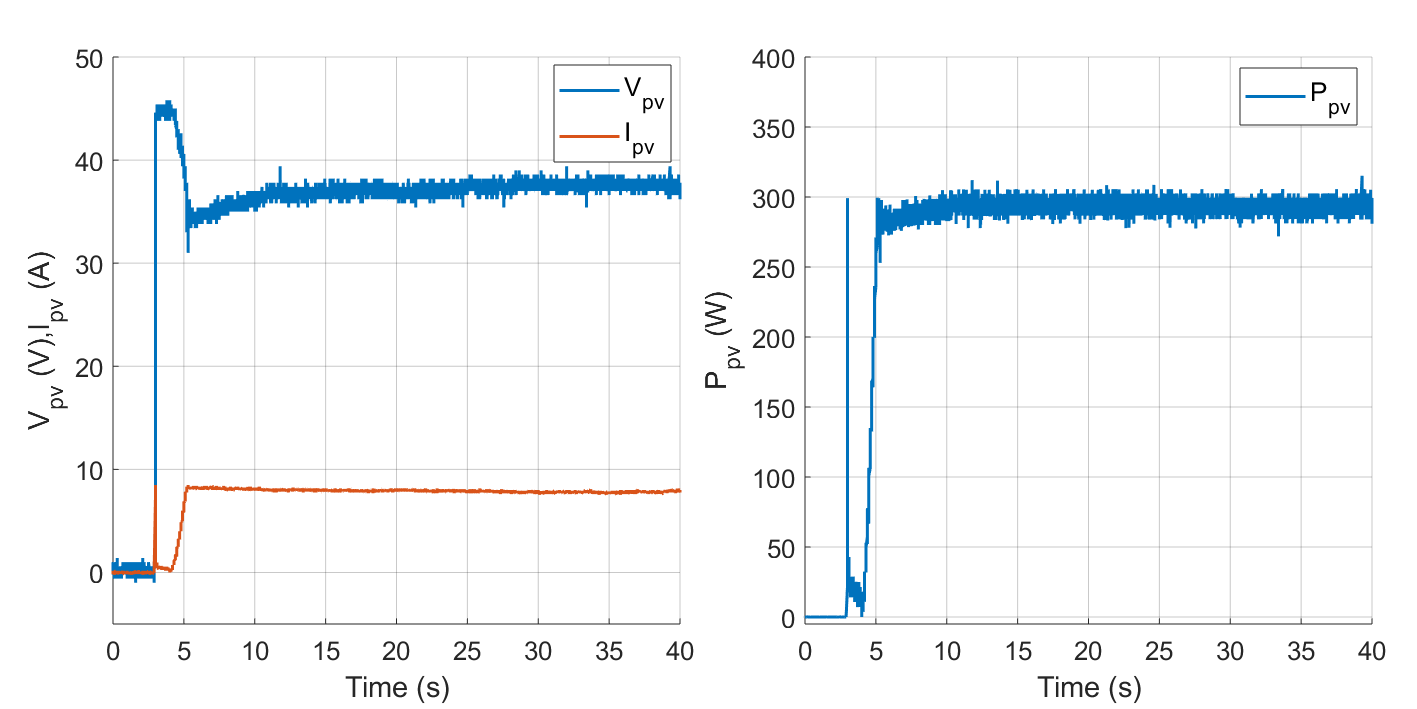
\includegraphics[width=1\textwidth]{../Pictures/P1/Test/Buck_mode_MPPT_Vin_Iin_Pin}
		\caption{Measured voltage, current and power extracted from the PV panel ($R_{L}=3\Omega$).}
		\label{MPPTtestbuckmode1}
	\end{center}	
\end{figure}

In the left graph in figure \ref{MPPTtestbuckmode2} it is observed the relationship between input and output voltage of the converter. From these measurements it is possible to calculate the duty cycle in buck mode for the optimal operating point as in equation \ref{eq:measureddutybuck}. 

\begin{equation} \label{eq:measureddutybuck}
D_{buck}= \dfrac{V_{out}}{V_{pv}} = \dfrac{28.29V}{37.25} = 0.7594
\end{equation}

The right graph shows the measured input and output power of the converter. From these measurements the efficiency of the converter is calculated in equation \ref{eq:effconverterbuck}.

\begin{equation} \label{eq:effconverterbuck}
\eta_{converter}= \dfrac{P_{out}}{P_{pv}} \cdot 100 = \dfrac{273.44W}{293.56W} \cdot 100 = 93.15\% 
\end{equation}


\begin{figure}[H]
	\begin{center}
		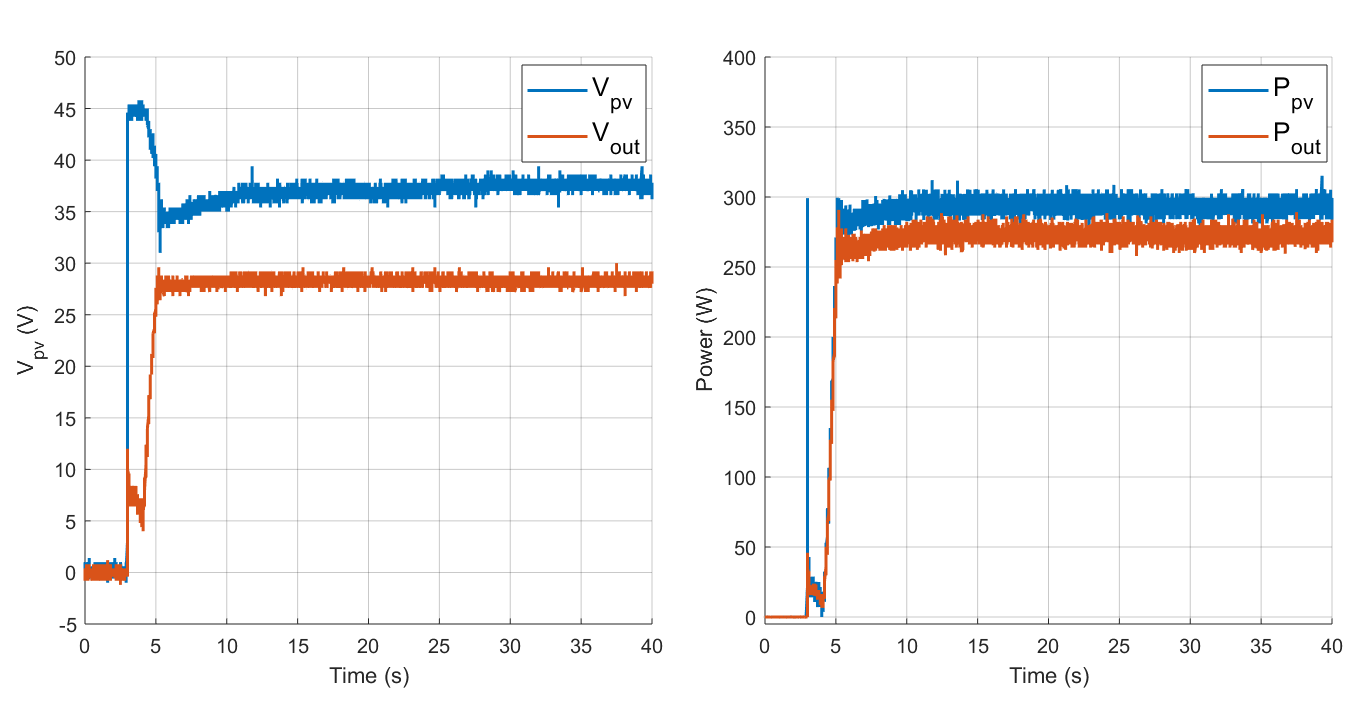
\includegraphics[width=1\textwidth]{../Pictures/P1/Test/Buck_mode_MPPT_Vin_Vout_Pin_Pout}
		\caption{Measured voltages and powers at the input and output of the converter ($R_{L}=3\Omega$).}
		\label{MPPTtestbuckmode2}
	\end{center}	
\end{figure}

Figure \ref{MPPTtestboostmode1} shows how the converter is tracking the MPP in boost mode. Here again is observed that the MPPT is enabled after the input voltage has reached the value of open-circuit. The time the MPPT takes to reach the MPP is higher than in buck mode, reaching it in 22 seconds \todo{approximately!Ask Thassilo for the exact value. Stef}. By comparing the measured power with the maximum power that the PV panel can generate under STC, the MPPT's efficiency is calculated in equation \ref{eq:effMPPTboost}. It is observed that even though the system needs more time to track the MPP it does not have a significant effect in the efficiency.

\begin{equation} \label{eq:effMPPTboost}
\eta_{MPPT}= \dfrac{P_{pv}}{P_{mpp}} \cdot 100 = \dfrac{292.37W}{300.4W} \cdot 100 = 97.32\%  
\end{equation}


\begin{figure}[H]
	\begin{center}
		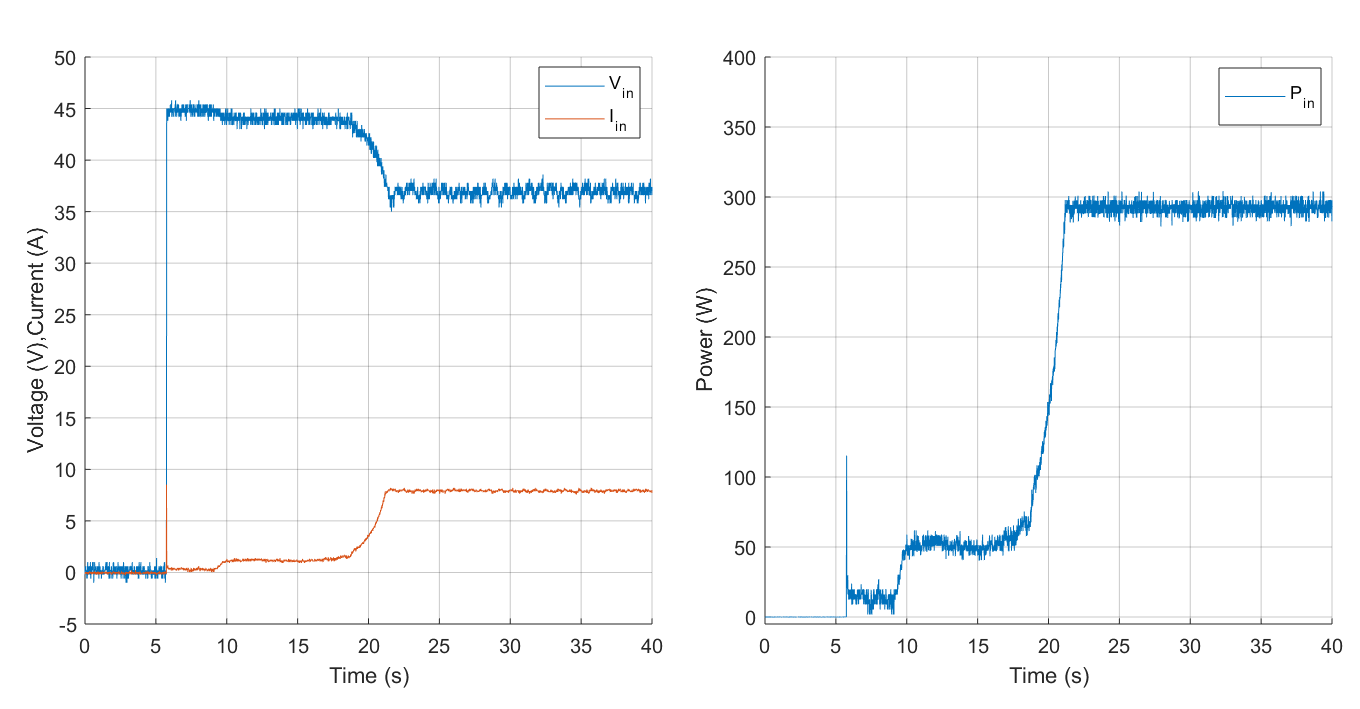
\includegraphics[width=1\textwidth]{../Pictures/P1/Test/Boost_mode_MPPT_Vin_Iin_Pin}
		\caption{Measured voltage, current and power extracted from the PV panel ($R_{L}=27\Omega$). picture not right! change axis labels and legend}
		\label{MPPTtestboostmode1}
	\end{center}	
\end{figure}

From the left graph of figure \ref{MPPTtestboostmode2} the duty cycle in boost mode for the optimal operating point can be calculated as in equation \ref{eq:measureddutyboost}. From the right graph the converter's efficiency is calculated as shown in equation \ref{eq:effconverterboost}.

\begin{equation} \label{eq:measureddutyboost}
D_{boost}= 1 - \dfrac{V_{pv}}{V_{out}} = 1 - \dfrac{36.93V}{88.41V} = 0.5823
\end{equation}

\begin{equation} \label{eq:effconverterboost}
\eta_{converter}= \dfrac{P_{out}}{P_{pv}} \cdot 100 = \dfrac{297.5W}{292.37W} \cdot 100 = 101.75\% 
\end{equation}
\todo{CHECK THIS AND DECIDE WHAT TO DO!! STEF}

\begin{figure}[H]
	\begin{center}
		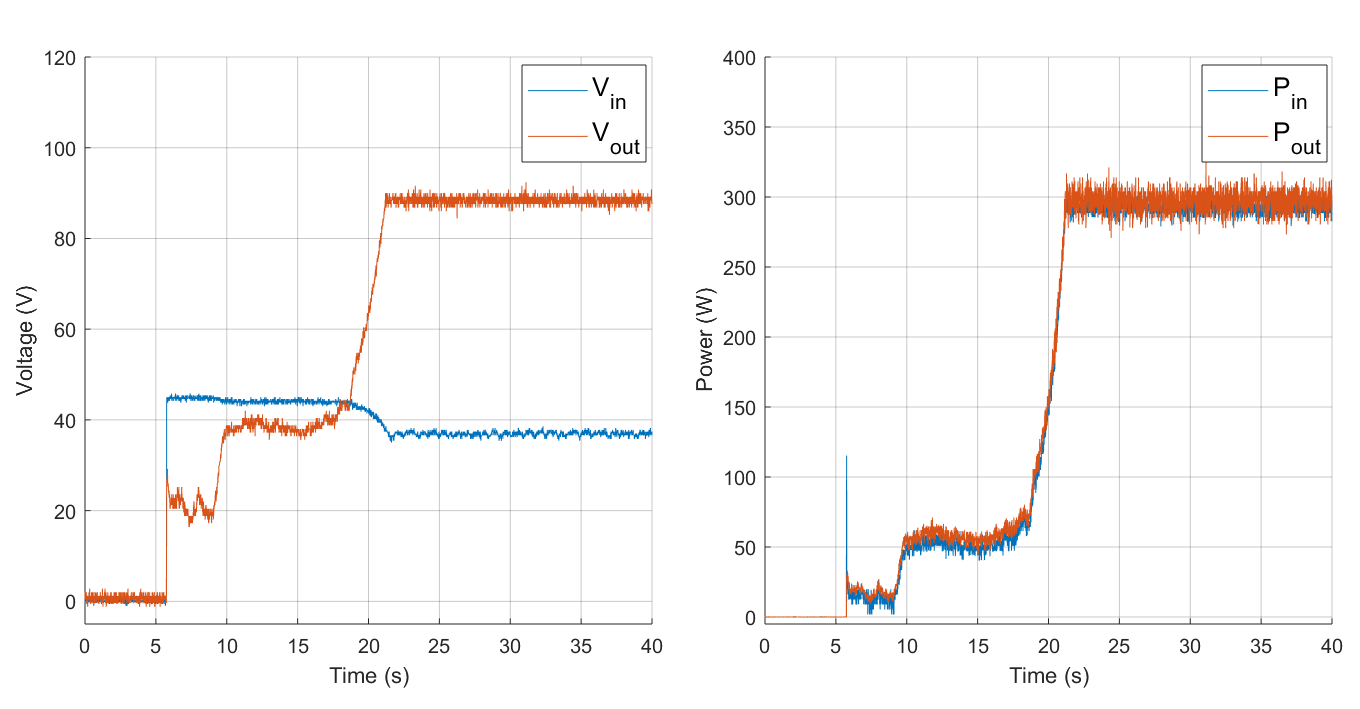
\includegraphics[width=1\textwidth]{../Pictures/P1/Test/Boost_mode_MPPT_Vin_Vout_Iin_Pin_Pout}
		\caption{Measured voltages and powers at the input and output of the converter ($R_{L}=27\Omega$).}
		\label{MPPTtestboostmode2}
	\end{center}	
\end{figure}



\subsubsection*{Change in irradiance and temperature}

HERE INCLUDE THE RESULTS FOR BUCK AND IN CASE WE GET TO DO BOOST ALSO HERE. 
